\section{HiTechnic NXT Compass Sensor}
Kompasset fra HiTechnic er et digitalt kompas der måler jordens magnetiske felt.
Kompasset kan returnere en værdi der repræsenterer kompassets nuværende orientering.
Ifølge HiTechnic er værdierne returneret fra kompasset præcise ned til 1 grad.
Kalibrering skulle desuden ikke være nødvendig.
Dog er det nødvendigt for at minimere forstyrrelser, at kompasset holdes 10-15 cm væk fra forstyrrende elementer, herunder \lego NXT og motorer.\cite{hitechnic_compass}

I \cref{kompas:precision} undersøges hvorvidt målinger fra kompasset kan leve op til disse oplysninger.

\subsection{Formål}
Formålet med denne test er at undersøge kompassets nøjagtighed.
Hvis kompasset har høj nøjagtighed kan det monteres på robotten og afgøre hvilken retning denne vender.

\subsection{Compass Sensor i \mindsqualls}
Til at styre denne sensor i \mindsqualls, skal der bruges en af de seperate klasser til HiTechnic sensorerne, som findes i namespacet \lstinline[style=csharp]!NXT.MindSqualls.HiTechnic!.
Til kompas sensoren anvendes klassen \lstinline[style=csharp]!HiTechnicCompassSensor!.

\subsubsection{Aflæsning af værdier}\label{kompas:reading}
Ved aflæsning af egenskaben \lstinline[style=csharp]!Heading! fra sensores klasse, gives et heltal mellem 0 og 359 der angiver kompassets orientering.
Det har været nødvendigt at ændre implementationen af \lstinline[style=csharp]!Heading!, da den oprindelige implementation ikke aflæste kompassets orientering ned til \'en grad.
Sensoren repræsenterer sin orientering på to forskellige måder.
Begge anvender to bytes.
Den ene metode beskriver afstanden vha. et 16-bit heltal.
Den anden (som var anvendt i implementationen af \lstinline[style=csharp]!Heading!) beskriver afstanden ved at lave den ene byte angive vinklen i intervaller af to grader.
Altså kunne de værdier der aflæses fra denne byte være 0-179, hvilket efterfølgende ganges med 2 for at få den egentlige værdi.
Hertil lægges værdien af den anden byte - der kan have værdien 0 eller 1.
I den oprindelige implementation af \lstinline[style=csharp]!Heading! er der ikke taget højde for denne ekstra værdi.
Dette er inddraget i test 3 i det følgende afsnit.

\subsection{Præcisionstest}\label{kompas:precision}
For at teste kompas sensoren, er målinger taget fra denne og holdt sammen med målinger foretaget med vinkelmåler.
Sammenligningen er sket ved at tage to målinger med kompasset, og sammenligne differencen med den værdi målt med vinkelmåler.
I forbindelse med test af sensoren blev der udført i alt tre tests:
\begin{enumerate}
\item Kompas monteret på robot med hjul
\item Kompas monteret på fast konstruktion
\item Gentagelse af test 2, med \textit{øget præcision}
\end{enumerate}
Den øgede præcision der beskrives her, dækker over en opdatering af \mindsqualls klassen \lstinline[style=csharp]!HiTechnicCompassSensor! der blev foretaget efter de første to tests.
Resultaterne fra de tre tests kan ses i tabellerne \ref{kompas:test1:table}, \ref{kompas:test2:table} og \ref{kompas:test3:table} på side \pageref{kompas:test1:table}.

Af resultaterne er der lavet et boksplot (\cref{kompas:boksplot}).
Plottet illustrerer den afvigelse der var fra de værdier der blev aflæst af kompasset, til de værdier der blev målt med vinkelmåler.
Prikkerne på plottet repræsenterer den gennemsnitlige afvigelse.

\begin{figure}[h]
\centering
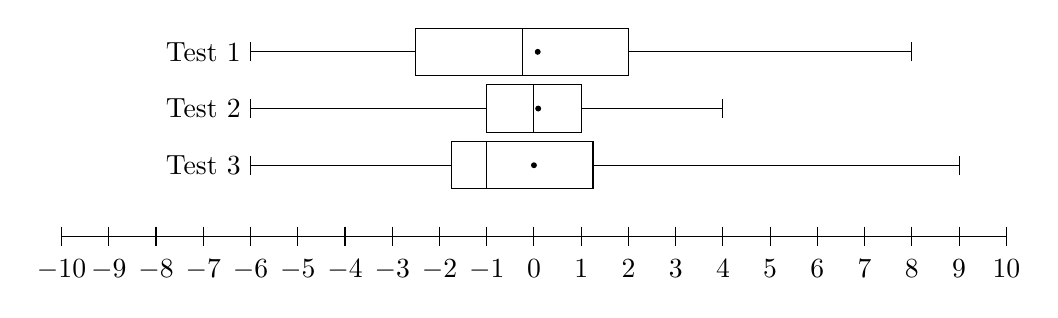
\begin{tikzpicture}[scale=0.6]
%Test 1
\draw (-2.5,3.4) rectangle (2,4.4); % Boks
\draw (-0.25,3.4) -- (-0.25,4.4); % Median streg
\draw (2,3.9) -- (8,3.9); % Fra øvre kvartil til maks
\draw (-2.5,3.9) -- (-6,3.9);% Fra nedre kvartil til min
\draw (8,3.7) -- (8,4.1); % Maksimum vertikal streg
\draw (-6,3.7) -- (-6,4.1); % Minimum vertikal streg
\node[left] at (-6,3.9) {Test 1};
\filldraw[color=black] (0.08,3.9) circle (0.05cm); % Gennemsnittet

%Test 2
\draw (-1,2.2) rectangle (1,3.2); % Boks
\draw (0,2.2) -- (0,3.2); % Median streg
\draw (1,2.7) -- (4,2.7); % Fra øvre kvartil til maks
\draw (-1,2.7) -- (-6,2.7);% Fra nedre kvartil til min
\draw (4,2.5) -- (4,2.9); % Maksimum vertikal streg
\draw (-6,2.5) -- (-6,2.9); % Minimum vertikal streg
\node[left] at (-6,2.7) {Test 2};
\filldraw[color=black] (0.09,2.7) circle (0.05cm); % Gennemsnittet

%Test 3
\draw (-1.75,1) rectangle (1.25,2); % Boks
\draw (-1,1) -- (-1,2); % Median streg
\draw (1.25,1.5) -- (9,1.5); % Fra øvre kvartil til maks
\draw (-1.75,1.5) -- (-6,1.5);% Fra nedre kvartil til min
\draw (9,1.3) -- (9,1.7); % Maksimum vertikal streg
\draw (-6,1.3) -- (-6,1.7); % Minimum vertikal streg
\node[left] at (-6,1.5) {Test 3};
\filldraw[color=black] (0.00,1.5) circle (0.05cm); % Gennemsnittet

% Linje med værdier
\draw (-10,0) -- (10,0);

% Tal på linje
\foreach \x in {-10,-9,...,10} {
	\draw (\x, 0.2) -- (\x, -0.2);
     \node[below] at (\x, -0.3) {$\x$};
}

\end{tikzpicture}
\caption{Boksplot for test af kompas}
\label{kompas:boksplot}
\end{figure}

\subsubsection{Test 1: Monteret på robot}
Første forsøg blev udført med kompasset monteret ovenpå ultralyds-sensoren, for at holde en minimum-afstand på 15 cm fra brick og motorer.
Denne konstruktion var dog meget ustabil, da kompasset skulle være forholdsvist højt oppe ift. base-konstruktionen.

\subsubsection{Test 2: Monteret på stabil konstruktion}
Andet forsøg blev udført med kompasset monteret på en selvstændig og langt mere stabil konstruktion, for derved at undersøge om dette kunne forbedre resultaterne.

\subsubsection{Test 3: Forøget præcision (stabil konstruktion)}
Tredje forsøg var en gentagelse af det andet, efter implementationen af \lstinline[style=csharp]!Heading! blev opdateret.
Målingerne her skulle altså udtrykke en øget præcision i forhold til den forrige test.
Det er valgt at medtage de første to tests, da forbedringen af præcisionen højst kunne være \'en grad ved denne tredje test (se \textit{\cref{kompas:reading}: \nameref*{kompas:reading}}).
Altså en marginal forbedring i forhold til testresultaterne.

\subsubsection{Resultater}
Som det fremgår af \cref{kompas:boksplot} er den gennemsnitlige afvigelse i alle tests meget tæt på 0.
Altså ved vi at kompasset lave lige mange og lige store (i gennemsnit) udsving til begge sider, hvilket gør det sværere at kalibrere for sådanne udsving.
Samtidig viser plottet, at halvdelen af kompassets målinger er over 2-3$\dg$ ved siden af de egentlige målinger - med den største afvigelse på 9$\dg$.

Det har i testfasen vist sig, at kompasset er konsistent i dets målinger.
Dette betyder at der ikke kan opnås yderligere præcision ved at foretage flere målinger af samme grad.
Disse målinger vil ganske enkelt give samme resultat.

Det kan hermed konkluderes at kompas sensoren ikke har høj nok præcision til at kunne anvendes i projektet.
